\chapter{Training Spiking Deep Learning Models On-line Using Spike-based Rate Multiplication (SRM)}
\label{cha:sdlm}
%Paragraph One: LINK
%Make a connection to what has immediately gone before. Recap the last chapter. In the last chapter I showed that… Having argued in the previous chapter that… As a result of x, which I established in the last chapter….. It is also possible to make a link between this chapter and the whole argument… The first step in answering my research question (repeat question) .. was to.. . In the last chapter I …
Having argued in the previous chapter that it is feasible to construct deep SNNs off-line by training DNN with specific activation function.
This Chapter continues the hot topic of deep SNNs and takes extra step forward to biologically inspired, on-line, spike-based training.

%Paragraph Two: FOCUS
%Now focus the reader’s attention on what this chapter is specifically going to do and why it is important. In this chapter I will examine.. I will present… I will report … This is crucial in (aim of thesis/research question) in order to….
In this Chapter We will present the method, Spike-based Rate Multiplication (SRM).
This algorithm successfully transfers multiplication operations to possibility of some specific firing events of a pair of rate-coded spike trains.
Moreover, these firing events can be captured with Synaptic-Time-Dependent Plasticity (STDP) rule thus to update the weights accordingly in an on-line, event-based, and biologically-plausible manner.
Such weights update well fits the conventional unsupervised deep learning modules: such as Autoencoders (AE) and Restricted Boltzmann Machines (RBMs), where multiplication of the neural outputs is the main operation.
It is crucial to provide deep SNNs with effective on-line training algorithm not only for building successful spike-based object recognition applications, but also for better power efficiency and scalability when training on neuromorphic hardware.


%Paragraph Three: OVERVIEW
%The third paragraph simply outlines the way that you are going to achieve the aim spelled out in the previous paragraph. It’s really just a statement of the contents in the order that the reader will encounter them. It is important to state these not simply as topics, but actually how they build up the internal chapter argument… I will begin by examining the definitions of, then move to seeing how these were applied… I first of all explain my orientation to the research process, positioning myself as a critical scholar.. I then explain the methodology that I used in the research, arguing that ethnography was the most suitable approach to provide answers to the question of… 
%https://patthomson.net/2014/01/16/connecting-chapterschapter-introductions/
We first of all explore the research question of on-line, event-based deep SNN training in the literature.
We then describe SRM in mathematical expression, and explain the factors influencing the accuracy of the method and the factors not. 
Afterwards we argue why the learning algorithm is proper to train spiking Autoencoders (SAEs) and Spiking Restricted Boltzmann Machines (SRBM).
During the research we encountered the problem introduced by the correlated spikes, therefore we also propose solutions to decorrelate spike trains in Section~\ref{sec:problem}. 
Finally the detailed comparison of the traditional training and SRM learning on MNIST dataset demonstrates the equivalent learning ability and shows similar even surpassing recognition and reconstruction capability of SRM.


\section{Related Works}
%To start with evidence of energy efficiency: maybe should refer to Chapter 2 or 1.
The current trend towards training deep SNNs on line using biologically-plausible learning methods is promising due to its potential benefit on low-energy hardware implementation.
%0. Dan Neil: Online Learning in Event-based Restricted Boltzmann Machines
The first on-line training algorithm of unsupervised learning is event-based contrastive divergence (evtCD)~\cite{neil2013online} for SRBM, which firstly found out the feasibility of applying STDP rule to approximate CD algorithm.
To review the algorithm of training RBMs, please refer to Section~\ref{sec:rbm}.
The method divided the learning process into potentiating and depression parts, which formed the basic design of related research.
As an initial attempt the mathematical analysis was mainly ignored, thus the best classification performance achieved was only about 81.5\% using purely spiking neurons.
%1. Neftci
\cite{neftci2013event} derived the division of potentiating and depression parts of CD algorithm, but conduct them both on the same neural populations which was more biologically plausible.
Therefore, a global signal was needed to differentiate the potentiating and depression process.
And the rhythmic oscillation of these processes generated the particular form of neural sampling~\cite{petrovici2013stochastic}.
The work focused on the statistical aspect of the event-driven sampling, and was extended to the later work on Synaptic Sampling Machines (S2Ms)~\cite{neftci2016stochastic} with stochastic synapses.
The classification accuracy of MNIST was 91.9\%, 1.7\% lower than the conventional RBM.
Similar work of Dan's SRBM training, \cite{burbank2015mirrored} applied STDP rule to train SAEs in very much biologically-plausible manner.
This work aimed at constructing artificial machine learning algorithm closely to biology, whereas the other works above focused on training spiking deep learning modules with equivalent recognition capability as alternative deep learning methods.

%4. remote (ReSuMe)
The work we propose was mostly inspired from the supervised time-based spiking learning rule~\cite{ponulak2010supervised}, ReSuMe, where the output spikes of a post-synaptic neuron were trained to generate at expected time points with certain input pattern injected to the pre-synaptic neurons, see Figure~\ref{fig:resume}.
The teaching signal always potentiates the synaptic strength according to the exponential STDP curve on the time difference between the teaching spike and the pre-synaptic spike; and the output spikes of the post-synaptic neuron always depress the connection.
Thus, if an output spike fires earlier than the teaching spike the weight will depress more than it potentiate, thus the output spike should be delayed the next trial; and the vice versa if the post-synaptic neuron spikes later.
Therefore, the weight stays constant only when the output spikes fire coincidently with the teaching signal.
\begin{figure}
	\centering
	\includegraphics[width=0.4\textwidth]{pics_sdlm/ReSuMe.pdf}
	\caption{Network architecture of a pair of pre- and post-synaptic neurons trained by ReSuMe~\cite{ponulak2010supervised} with a teaching signal.}
	\label{fig:resume}
\end{figure}

The basic idea of the proposed method is to provide equivalent learning rule as ReSuMe on rate-encoded SNNs.
The objective is to supervise the post-synaptic neuron to fire at the frequency of the teaching spike train. 
Accordingly, the weight decreases if the output neuron fires stronger than the teaching neuron, and vice versa.
The synaptic strength stops changing as the output neuron fires at the same frequency of the teaching signal.
The algorithm is simply divided into spike-based rate multiplication (SRM) problems, and we will demonstrate the SRM method in following Section~\ref{sec:SRM}.
The learning rule can be easily applied to SAEs if we use input spikes as teaching signals to the visible units, moreover the CD algorithm of training SRBMs is still not more than two operations of SRMs.
Section~\ref{sec:dSNN} explains the specific training on SAEs and SRBMs in detail.
 

\section{Spike-based Rate Multiplication (SRM)}
\label{sec:SRM}
If we see \textit{pre}, \textit{post} and \textit{teach} as vectors individually, and \textit{w} as a weight matrix of the all-to-all connections between \textit{pre} and \textit{post} in Figure~\ref{fig:resume}, the network will form the Adaline (Adaptive Linear Element) which is a single-layered ANN.
The learning algorithm was named after the researcher Widrow-Hoff:
\begin{equation}
\Delta w = \eta (teach - post)pre,
\end{equation}
which is equivalent to Stochastic Gradient Descent~(SGD) in Multi-Layered Perceptrons~(MLPs).
The right hand of the equation can be seen as two operations of multiplication, $teach \times pre$ and $post \times pre$, times the constant learning rate, $\eta$.

SRM provides the solution to present numeric multiplication $c=ab$ with rate-based spike trains.
First of all, the multiplier $a$ and the multiplicand $b$ are encoded into Poisson spike trains $s_a=\{s_a(1),s_a(2),...,s_a(T)\}$ and $s_b=\{s_b(1),s_b(2),...,s_b(T)\}$ in the 1~ms resolution, where $s(t)=1$ indicates a spike in the $t$th~ms and $s(t)=0$ means none.
Secondly, a Poisson generator fires a sequence of spike train according to its firing rate, $\lambda$~Hz, which is assigned linearly to the original multiplier/multiplicand by a factor of $K$.
Hence, the firing rate ($\lambda_x$) of the Poisson generator is $K$ times of the numerical value x, and can be approximated by the average spike count, $N_T(s_x)$, of the generated spike train $s_x$ over time length of $T$:
\begin{equation}
\lambda_x = Kx \approx N_T(s_x) = \frac{1000}{T} \sum_{t=1}^{T} s_x(t) ,
\end{equation} 
and 1000 is the scale factor for scaling frequency per millisecond to per second.
Significantly, the approximation is more accurate as the observing time ($T$) grows since more spikes are generated over time and the average spike count becomes more reliable.
Thirdly, assuming $s_a$ and $s_b$ are independent Poisson spike trains the core definition of the rate multiplication of the pair of spike trains is as follows:
\begin{equation}
\lambda_a \lambda_b \approx N_{T_1}(s_a)N_{T_2}(s_b)= 10^6 \frac{\sum_{t_a=1}^{T_1}s_a(t_a)}{T_1}  \frac{\sum_{t_b=1}^{T_2} s_b(t_b)}{T_2}.
\label{equ:mul}
\end{equation} 

Finally, if we combine the concept of the STDP learning window to equation~\ref{equ:mul}, the length of the observing time on $s_b$ shrinks to a fix-length windowing period, $\tau_{win}$.
Consequently, the rate multiplication can be conducted within only the local events in term of time, although the accuracy may drop.
The rate multiplication is then approximated by:
\begin{equation}
\lambda_a \lambda_b \approx \frac{10^6}{\tau_{dur} \tau_{win}} \sum_{t=1}^{\tau_{dur}} [s_a(t) \sum_{t_b=t}^{t+\tau_{win}} s_b(t_b)],
\end{equation} 
where $\tau_{dur}$ replaces $T$ to represent the length of generated spike trains during SNN simulation.
The weight rise/drop according to a rectangular STDP curve can detect the spike events of a pair of spike trains when post-synaptic spike occurs no later than $\tau_{win}$, see Figure~\ref{fig:rtg_stdp}.
Therefore, the overall weight change during time $\tau_{dur}$ indicates the rate multiplication, and is decried by SRM:
\begin{equation}
\begin{aligned}
\Delta w &= \eta_s \sum_{t=1}^{\tau_{dur}} [s_a(t) \sum_{t_b=t}^{t+\tau_{win}} s_b(t_b)] \text{, and}\\
c=ab=\frac{\lambda_a \lambda_b}{K^2} &\approx \frac{10^6}{K^2 \tau_{dur} \tau_{win}} \sum_{t=1}^{\tau_{dur}} [s_a(t) \sum_{t_b=t}^{t+\tau_{win}} s_b(t_b)] \\
&\approx  \frac{10^6 \Delta w}{K^2 \tau_{dur} \tau_{win}  \eta_s}.
\end{aligned}
\end{equation} 
\begin{figure}
	\centering
	\includegraphics[width=0.4\textwidth]{pics_sdlm/stdp.pdf}
	\caption{Rectangular STDP curve.
		If the time difference of the post-synaptic spike and the pre-synaptic spike lies in the window on $\tau_{win}$, then the synaptic weight will increase by $\eta_s$.}
	\label{fig:rtg_stdp}
\end{figure}

We can adjust $\eta_s$ to $ K^2 \tau_{dur} \tau_{win}10^{-6}$ to make $ab = \Delta w$.
In terms of the Widrow-Hoff learning algorithm, $\eta_s$ is set to be:
\begin{equation}
	\eta_s=
    \left\{
    \begin{aligned} 
    \eta K^2 \tau_{dur} \tau_{win}10^{-6}, &\text{ when calculating } \eta teach \times pre\\
    - \eta K^2 \tau_{dur} \tau_{win}10^{-6}, &\text{ when calculating } \eta post \times pre
    \end{aligned}
    \right.
\end{equation}
In Section~\ref{sec:AE}, we demonstrate how Widrow-Hoff algorithm successfully applies to training AEs (see Equation~\ref{equ:ae_widrow_hoff}) and in the next section we describe the implementation of SRM algorithm to deep learning models of spiking AEs and RBMs.

Last but not least, we state the property of SRM algorithm:
\begin{itemize}
	\item the accuracy of SRM is mainly controlled by $\tau_{dur}$ and $\tau_{win}$, where longer spike trains and longer STDP window expresses the rate more reliable.
	\item in spiking neural network both the multiplier and the multiplicand can only be presented as rates, which is positive.
	Thus negative product is applied with weight decrease, $-\eta_s$. 
	\item the multiplier and the multiplicand are interchangeable due to the independence of the spike trains. 
	\item the accuracy is independent of neural model and synaptic model because the calculation replies on the firing rate only.
\end{itemize}
\section{Training Deep SNNs}
\label{sec:dSNN}
The Section conducts experiments to compare conventional deep learning modules to spiking versions of them.
To start with, AEs and RBMs are trained with clean numerical values, and then with noisy values which are generated by presenting the original values with Poisson spike trains and transferring the spike counts back to numerical values.
These experiments run as baselines to compare with spike based training on the features of weights' convergence, reconstruction error and neurons' activities.

There are two set-ups of the same network architecture where ten visible neurons connect to the layer of ten hidden neurons symmetrically with all-to-all weights: (1)~the values of all the input data are 1, $input_1 = [1, 1, 1,...,1]$; and (2)~the input data range from 0.1 to 1 linearly with step of 0.1, $input_2 = [0.1, 0.2, 0.3,...,1]$.
These two experiments provide a close observation on the weight updates given the constant input values.
And Experiment I shows how the network responds to a same input value 1, and reconstructs it; while Experiments II can demonstrate the influence of ranging input values, more importantly how firing rate may affect the corresponding SNN.

Following the experiments of conventional models, we propose the training methods of SAEs and SRBMs in detail.
The same experiments are then applied to the on-line and spike-based algorithm.

\subsection{Autoencoders (AEs)}
Using ReLU and Equation~\ref{equ:ae_widrow_hoff}, we can easily train a layer of AEs with a small network size of 10 visible units and 10 output units.
The initial weights are randomly generated with unified distribution from 0 to 0.01, and the learning rate, $\eta$, is set to 0.001.
We keep the same initial weights for all the experiments thus to provide an accurate comparison on the weights update.
The input vector, seen as an image, repeatedly feed into the network for $5,000$ times and Figure~\ref{fig:ae_orig} shows the dynamics of the AE as more repeating images present through training.

\begin{figure}
	\centering
	\begin{subfigure}[t]{0.45\textwidth}
		\includegraphics[width=\textwidth]{pics_sdlm/20_exp_AE/exp1_weights_non.pdf}
		\caption{Weights of Exp1}
	\end{subfigure}
	\begin{subfigure}[t]{0.45\textwidth}
		\includegraphics[width=\textwidth]{pics_sdlm/20_exp_AE/exp2_weights_non.pdf}
		\caption{Weights of Exp2}
	\end{subfigure}
	\begin{subfigure}[t]{0.45\textwidth}
		\includegraphics[width=\textwidth]{pics_sdlm/20_exp_AE/exp1_recon_non.pdf}
		\caption{Reconstruction of visible units in Exp1}
	\end{subfigure}
	\begin{subfigure}[t]{0.45\textwidth}
		\includegraphics[width=\textwidth]{pics_sdlm/20_exp_AE/exp2_recon_non.pdf}
		\caption{Reconstruction of visible units in Exp2}
	\end{subfigure}\\
	\begin{subfigure}[t]{0.45\textwidth}
		\includegraphics[width=\textwidth]{pics_sdlm/20_exp_AE/exp1_hid_non.pdf}
		\caption{Output of hidden units in Exp1}
	\end{subfigure}
	\begin{subfigure}[t]{0.45\textwidth}
		\includegraphics[width=\textwidth]{pics_sdlm/20_exp_AE/exp2_hid_non.pdf}
		\caption{Output of hidden units in Exp2}
	\end{subfigure}\\
	\begin{subfigure}[t]{0.45\textwidth}
		\includegraphics[width=\textwidth]{pics_sdlm/20_exp_AE/exp1_loss.pdf}
		\caption{Output of hidden units in Exp1}
	\end{subfigure}
	\begin{subfigure}[t]{0.45\textwidth}
		\includegraphics[width=\textwidth]{pics_sdlm/20_exp_AE/exp2_loss.pdf}
		\caption{Output of hidden units in Exp2}
	\end{subfigure}
	\caption{Changes of weights, output of visible and hidden units, and mean squared error (loss) during the AE training of the reconstruction tests. 
		Experiments 1) 10 visible units fully connected to 10 hidden units with input data of all 1s; 2) same network fed with 10 values distribute linearly from 0.1 to 1.}
	\label{fig:ae_orig}
\end{figure}

In order to compare all the experiments following, we demonstrate the results in the same figure template:
(a) and (b) depict the weights change of the two experiment set-ups (Exp1 and Exp2) which is the most important output of a training method;
(c) and (d) visually display the output of the visible units, the reconstruction of the input vector;
(e) and (f) draw the output of the hidden units during training and assist the observation on weight change and the reconstruction;
(g) and (h) intuitively show the loss (mean squared error) and validate how well the reconstructions are.


For Exp1, the reconstruction loss reduces exponentially to the limit of the computer's float precision (Figure~\ref{fig:ae_orig}(g)), and reaches $10^{-4}$ using about 600 steps, and from that point the weights, visible reconstruction, and the output of the hidden units nearly stabilise, see Figure~\ref{fig:ae_orig}(a,c,e).
With differentiate input values in Exp2, the training runs slower taking about $1,400$ steps to reach the same performance of $10^{-4}$ loss (Figure~\ref{fig:ae_orig}(h)).
The reason of the slower training comes to the weaker input and it also makes the output of the hidden units lower than Exp1, see Figure~\ref{fig:ae_orig}(f), thus the positive part of the weight change, $\eta h_i v_j$, is much weakened. 
The reconstructions, shown in Figure~\ref{fig:ae_orig}(d), of smaller values stabilise earlier than the ones of higher values, since the higher output of the reconstruction requires stronger weights and more accumulated weights update. 
\begin{figure}
	\centering
	\begin{subfigure}[t]{0.45\textwidth}
		\includegraphics[width=\textwidth]{pics_sdlm/21_exp_AE_noise/exp1_weights_s.pdf}
		\caption{Weights of Exp1}
	\end{subfigure}
	\begin{subfigure}[t]{0.45\textwidth}
		\includegraphics[width=\textwidth]{pics_sdlm/21_exp_AE_noise/exp2_weights_s.pdf}
		\caption{Weights of Exp2}
	\end{subfigure}
	\begin{subfigure}[t]{0.45\textwidth}
		\includegraphics[width=\textwidth]{pics_sdlm/21_exp_AE_noise/exp1_recon_s.pdf}
		\caption{Reconstruction of visible units in Exp1}
	\end{subfigure}
	\begin{subfigure}[t]{0.45\textwidth}
		\includegraphics[width=\textwidth]{pics_sdlm/21_exp_AE_noise/exp2_recon_s.pdf}
		\caption{Reconstruction of visible units in Exp2}
	\end{subfigure}\\
	\begin{subfigure}[t]{0.45\textwidth}
		\includegraphics[width=\textwidth]{pics_sdlm/21_exp_AE_noise/exp1_hid_s.pdf}
		\caption{Output of hidden units in Exp1}
	\end{subfigure}
	\begin{subfigure}[t]{0.45\textwidth}
		\includegraphics[width=\textwidth]{pics_sdlm/21_exp_AE_noise/exp2_hid_s.pdf}
		\caption{Output of hidden units in Exp2}
	\end{subfigure}\\
	\begin{subfigure}[t]{0.45\textwidth}
		\includegraphics[width=\textwidth]{pics_sdlm/21_exp_AE_noise/exp1_loss_s.pdf}
		\caption{Output of hidden units in Exp1}
	\end{subfigure}
	\begin{subfigure}[t]{0.45\textwidth}
		\includegraphics[width=\textwidth]{pics_sdlm/21_exp_AE_noise/exp2_loss_s.pdf}
		\caption{Output of hidden units in Exp2}
	\end{subfigure}
	\caption{Changes of weights, output of visible and hidden units, and mean squared error (loss) during the AE training of the noisy reconstruction tests. 
		Experiments 1) 10 visible units fully connected to 10 hidden units with the count of Poisson spikes firing at 100~Hz which lasted 100~ms; 2) same network fed with spike count of Poisson spikes at firing rate ranging from 10~Hz to 100~Hz.}
	\label{fig:ae_noise}
\end{figure}

The same experiments are repeated with noisy training and testing data to provide a fair comparison with the spike-based deep learning modules, see Figure~\ref{fig:ae_noise}.
The noisy data is gathered from the SNN experiments in Section~\ref{subsec:SAE}, and the corresponding SRM parameters are listed in Table~\ref{tbl:srm}.
All the SNN experiments use the same training and testing Poisson spike trains for the purpose of unified experimental environment.
The firing rates of the input values are scaled up by the factor $K = 100$, thus $\lambda_1 = [100, 100, 100, ..., 100]$ Hz and $\lambda_2 = [10, 20, 30, ..., 100]$ Hz.
The spike count $c$ of a generated Poisson spike train then transformed to the noisy input, $c/(\tau_{dur} * K)$.
The length of spike trains $\tau_{dur}$ is 0.1~s when training, and 1~s for testing.
The longer the spike trains are, less noisy the spike counts become.
The noisy input can be seen as distorted data by adding Gaussian noise on the original value.
Hence, the noisy training input adds the clean data a Gaussian noise with -0.05 mean and 0.29 variance for Exp1, and -0.02 mean and 0.22 variance for Exp2;
while in terms of testing data, see Figure~\ref{fig:noise_input}, the means of the noise are the same, but the variances are much smaller: 0.09 for Exp1 and 0.07 for Exp2.
\begin{figure}
	\centering
	\begin{subfigure}[t]{0.45\textwidth}
		\includegraphics[width=\textwidth]{pics_sdlm/21_exp_AE_noise/exp1.pdf}
		\caption{Input images of Exp1}
	\end{subfigure}
	\begin{subfigure}[t]{0.45\textwidth}
		\includegraphics[width=\textwidth]{pics_sdlm/21_exp_AE_noise/exp2.pdf}
		\caption{Input images of Exp2}
	\end{subfigure}
	\caption{Noisy input gathered from Poisson spike trains.}
	\label{fig:noise_input}
\end{figure}


Figure~\ref{fig:ae_noise} shows the effect of the noisy input, although the training stabilises at roughly the same time point.
First of all, it generates slight waves on the weight changes.
Secondly, the reconstruction and the output of the hidden units are noisy comparing to the training and testing on clean data, however the noise are much reduced from the noisy input data (Figure~\ref{fig:noise_input}). 
Finally, the loss keeps in a certain level and stops dropping.
The loss of Exp2 is lower than Exp1, in other words the reconstruction on Exp2 are closer to the input data.
It is mainly caused the weaker noise level on the smaller input values that the data is less noisy in Exp2 in average. 
\begin{figure}
	\centering
	\begin{subfigure}[t]{0.4\textwidth}
		\includegraphics[width=\textwidth]{pics_sdlm/30_exp_RBM/exp1_weights_non.pdf}
		\caption{Weights of Exp1}
	\end{subfigure}
	\begin{subfigure}[t]{0.4\textwidth}
		\includegraphics[width=\textwidth]{pics_sdlm/30_exp_RBM/exp2_weights_non.pdf}
		\caption{Weights of Exp2}
	\end{subfigure}
	\begin{subfigure}[t]{0.4\textwidth}
		\includegraphics[width=\textwidth]{pics_sdlm/30_exp_RBM/exp1_recon_non.pdf}
		\caption{Reconstruction of visible units in Exp1}
	\end{subfigure}
	\begin{subfigure}[t]{0.4\textwidth}
		\includegraphics[width=\textwidth]{pics_sdlm/30_exp_RBM/exp2_recon_non.pdf}
		\caption{Reconstruction of visible units in Exp2}
	\end{subfigure}\\
	\begin{subfigure}[t]{0.4\textwidth}
		\includegraphics[width=\textwidth]{pics_sdlm/30_exp_RBM/exp1_hid_non.pdf}
		\caption{Output of hidden units in Exp1}
	\end{subfigure}
	\begin{subfigure}[t]{0.4\textwidth}
		\includegraphics[width=\textwidth]{pics_sdlm/30_exp_RBM/exp2_hid_non.pdf}
		\caption{Output of hidden units in Exp2}
	\end{subfigure}\\
	\begin{subfigure}[t]{0.4\textwidth}
		\includegraphics[width=\textwidth]{pics_sdlm/30_exp_RBM/exp1_loss.pdf}
		\caption{Output of hidden units in Exp1}
	\end{subfigure}
	\begin{subfigure}[t]{0.4\textwidth}
		\includegraphics[width=\textwidth]{pics_sdlm/30_exp_RBM/exp2_loss.pdf}
		\caption{Output of hidden units in Exp2}
	\end{subfigure}
	\caption{Changes of weights, output of visible and hidden units, and mean squared error (loss) during the nRBM training of the reconstruction tests. 
		Experiments 1) 10 visible units fully connected to 10 hidden units with input data of all 1s; 2) same network fed with 10 values distribute linearly from 0.1 to 1.}
	\label{fig:rbm_orig}
\end{figure}

\subsection{Noisy Restricted Boltzmann Machines (nRBMs)}
Instead of using binary units in RBM, we employ noisy ReLU units constructing noisy RBM which is closer to biology and performs better in classification tasks~\cite{nair2010rectified}.
Leaving the learning algorithm unchanged, see Algorithm~\ref{alg:rbm} in Section~\ref{sec:rbm}, the new sampling method noisy ReLU (NReLU) is equivalent to generating multiple samples in the meantime and averaging them: $max(0, x+\mathcal{N}(0, \sigma(x))$.
The lower the variance of the normal distribution is, it means more samples are taken for averaging.
To put it differently, zero variance is used when unlimited samples are generated, but at the same time the sampling itself loses the randomness.
In our experiments the variance of the normal distribution used in NReLU is 0.1.







\begin{figure}
	\centering
	\begin{subfigure}[t]{0.4\textwidth}
		\includegraphics[width=\textwidth]{pics_sdlm/31_exp_RBM_noise/exp1_weights_s.pdf}
		\caption{Weights of Exp1}
	\end{subfigure}
	\begin{subfigure}[t]{0.4\textwidth}
		\includegraphics[width=\textwidth]{pics_sdlm/31_exp_RBM_noise/exp2_weights_s.pdf}
		\caption{Weights of Exp2}
	\end{subfigure}
	\begin{subfigure}[t]{0.4\textwidth}
		\includegraphics[width=\textwidth]{pics_sdlm/31_exp_RBM_noise/exp1_recon_s.pdf}
		\caption{Reconstruction of visible units in Exp1}
	\end{subfigure}
	\begin{subfigure}[t]{0.4\textwidth}
		\includegraphics[width=\textwidth]{pics_sdlm/31_exp_RBM_noise/exp2_recon_s.pdf}
		\caption{Reconstruction of visible units in Exp2}
	\end{subfigure}\\
	\begin{subfigure}[t]{0.4\textwidth}
		\includegraphics[width=\textwidth]{pics_sdlm/31_exp_RBM_noise/exp1_hid_s.pdf}
		\caption{Output of hidden units in Exp1}
	\end{subfigure}
	\begin{subfigure}[t]{0.4\textwidth}
		\includegraphics[width=\textwidth]{pics_sdlm/31_exp_RBM_noise/exp2_hid_s.pdf}
		\caption{Output of hidden units in Exp2}
	\end{subfigure}\\
	\begin{subfigure}[t]{0.4\textwidth}
		\includegraphics[width=\textwidth]{pics_sdlm/31_exp_RBM_noise/exp1_loss_s.pdf}
		\caption{Output of hidden units in Exp1}
	\end{subfigure}
	\begin{subfigure}[t]{0.4\textwidth}
		\includegraphics[width=\textwidth]{pics_sdlm/31_exp_RBM_noise/exp2_loss_s.pdf}
		\caption{Output of hidden units in Exp2}
	\end{subfigure}
	\caption{Changes of weights, output of visible and hidden units, and mean squared error (loss) during the nRBM training of the reconstruction tests. 
		Experiments 1) 10 visible units fully connected to 10 hidden units with the count of Poisson spikes firing at 100~Hz which lasted 100~ms; 2) same network fed with 10 count of Poisson spikes at firing rate ranging from 10~Hz to 100~Hz.}
	\label{fig:rbm_noise}
\end{figure}
The experiments on noisy input driven by Poissonian spike trains.
Figure~\ref{fig:ae_noise} and Figure~\ref{fig:rbm_noise} show how noise influence the training and output of both the visible and hidden units.
The change of the weights oscillates more. % and the value of the weights tends to diverge slightly as training goes on. 

\subsection{Training Spiking Autoencoders}
\label{subsec:SAE}
\begin{table}[hbbp]
	\centering
	\caption{\label{tbl:srm}Parameter setting of SRM for training SAEs and SRBMs.}
	\bgroup
	\def\arraystretch{1.4}
	\begin{tabular}{c c l}
		%\hline
		Parameters & Values & Description \\
		\hline
		K & 100 & linear scaling factor\\
		%\hline
		$\tau_{dur}$ & 100 ms &  length of training spike trains\\
		%\hline
		$\tau_{win}$ & 10 ms & window length of STDP\\
		%\hline
		$\eta$ & $10^{-3}$ & learning rate of AEs and RBMs\\
		%\hline
		$\eta_s$ & $10^{-4}$ nA & learning rate of SAEs and SRBMs\\
		%\hline
	\end{tabular}
	\egroup
\end{table}
\begin{figure}
	\centering
	\includegraphics[width=0.8\textwidth]{pics_sdlm/rSTDP.pdf}
	\caption{How rSTDP works in training spiking Autoencoders.}
	\label{fig:rSTDP}
\end{figure}

\subsection{Training Spiking RBM}
\begin{figure}
	\centering
	\includegraphics[width=0.8\textwidth]{pics_sdlm/rSTDP_rbm.pdf}
	\caption{How rSTDP works in training spiking RBMs.}
	\label{fig:rSTDP_rbm}
\end{figure}

\section{Problem}
\label{sec:problem}
Correlations in spike trains make weights diverge.
Experiments
\begin{figure}
	\centering
	\begin{subfigure}[t]{0.4\textwidth}
		\includegraphics[width=\textwidth]{pics_sdlm/00_exp_SAE_Orig/exp1_weights_s.pdf}
		\caption{Weights of Exp1}
	\end{subfigure}
	\begin{subfigure}[t]{0.4\textwidth}
		\includegraphics[width=\textwidth]{pics_sdlm/00_exp_SAE_Orig/exp2_weights_s.pdf}
		\caption{Weights of Exp2}
	\end{subfigure}
	\begin{subfigure}[t]{0.4\textwidth}
		\includegraphics[width=\textwidth]{pics_sdlm/00_exp_SAE_Orig/exp1_recon_s.pdf}
		\caption{Reconstruction of visible units in Exp1}
	\end{subfigure}
	\begin{subfigure}[t]{0.4\textwidth}
		\includegraphics[width=\textwidth]{pics_sdlm/00_exp_SAE_Orig/exp2_recon_s.pdf}
		\caption{Reconstruction of visible units in Exp2}
	\end{subfigure}\\
	\begin{subfigure}[t]{0.4\textwidth}
		\includegraphics[width=\textwidth]{pics_sdlm/00_exp_SAE_Orig/exp1_hid_s.pdf}
		\caption{Output of hidden units in Exp1}
	\end{subfigure}
	\begin{subfigure}[t]{0.4\textwidth}
		\includegraphics[width=\textwidth]{pics_sdlm/00_exp_SAE_Orig/exp2_hid_s.pdf}
		\caption{Output of hidden units in Exp2}
	\end{subfigure}\\
	\begin{subfigure}[t]{0.4\textwidth}
		\includegraphics[width=\textwidth]{pics_sdlm/00_exp_SAE_Orig/exp1_mse_nons.pdf}
		\caption{Loss of Exp1}
	\end{subfigure}
	\begin{subfigure}[t]{0.4\textwidth}
		\includegraphics[width=\textwidth]{pics_sdlm/00_exp_SAE_Orig/exp2_mse_nons.pdf}
		\caption{Loss of Exp2}
	\end{subfigure}
	\caption{Weights and firing rates of visible and hidden units change during training of the reconstruction tests of spiking AE. 
		Experiments 1) 10 visible units fully connected to 10 hidden units with Poisson spike trains of 100~Hz which lasted 100~ms; 2) same network fed with 10 Poisson spike trains of firing rate ranging from 10~Hz to 100~Hz.}
\end{figure}

\begin{figure}
	\centering
	\begin{subfigure}[t]{0.4\textwidth}
		\includegraphics[width=\textwidth]{pics_sdlm/10_exp_SRBM_Orig/exp1_weights_s.pdf}
		\caption{Weights of Exp1}
	\end{subfigure}
	\begin{subfigure}[t]{0.4\textwidth}
		\includegraphics[width=\textwidth]{pics_sdlm/10_exp_SRBM_Orig/exp2_weights_s.pdf}
		\caption{Weights of Exp2}
	\end{subfigure}
	\begin{subfigure}[t]{0.4\textwidth}
		\includegraphics[width=\textwidth]{pics_sdlm/10_exp_SRBM_Orig/exp1_recon_s.pdf}
		\caption{Reconstruction of visible units in Exp1}
	\end{subfigure}
	\begin{subfigure}[t]{0.4\textwidth}
		\includegraphics[width=\textwidth]{pics_sdlm/10_exp_SRBM_Orig/exp2_recon_s.pdf}
		\caption{Reconstruction of visible units in Exp2}
	\end{subfigure}\\
	\begin{subfigure}[t]{0.4\textwidth}
		\includegraphics[width=\textwidth]{pics_sdlm/10_exp_SRBM_Orig/exp1_hid_s.pdf}
		\caption{Output of hidden units in Exp1}
	\end{subfigure}
	\begin{subfigure}[t]{0.4\textwidth}
		\includegraphics[width=\textwidth]{pics_sdlm/10_exp_SRBM_Orig/exp2_hid_s.pdf}
		\caption{Output of hidden units in Exp2}
	\end{subfigure}\\
	\begin{subfigure}[t]{0.4\textwidth}
		\includegraphics[width=\textwidth]{pics_sdlm/10_exp_SRBM_Orig/exp1_mse_nons.pdf}
		\caption{Loss of Exp1}
	\end{subfigure}
	\begin{subfigure}[t]{0.4\textwidth}
		\includegraphics[width=\textwidth]{pics_sdlm/10_exp_SRBM_Orig/exp2_mse_nons.pdf}
		\caption{Loss of Exp2}
	\end{subfigure}
	\caption{Weights and firing rates of visible and hidden units change during training of the reconstruction tests of spiking RBM. 
		Experiments 1) 10 visible units fully connected to 10 hidden units with Poisson spike trains of 100~Hz which lasted 100~ms; 2) same network fed with 10 Poisson spike trains of firing rate ranging from 10~Hz to 100~Hz.}
\end{figure}

\subsection{Solution 1: Longer STDP Window}
The stronger correlation of a pair of pre- and post-synaptic neurons make the spikes generated by the post-synaptic neuron lie in the shorter period after the pre-synaptic spike.
So a longer square STDP window maker the overall weight change more dependent of the correlation of the spike trains.
\begin{figure}
	\centering
	\begin{subfigure}[t]{0.4\textwidth}
		\includegraphics[width=\textwidth]{pics_sdlm/01_exp_SAE_Orig_long/exp1_weights_s.pdf}
		\caption{Weights of Exp1}
	\end{subfigure}
	\begin{subfigure}[t]{0.4\textwidth}
		\includegraphics[width=\textwidth]{pics_sdlm/01_exp_SAE_Orig_long/exp2_weights_s.pdf}
		\caption{Weights of Exp2}
	\end{subfigure}
	\begin{subfigure}[t]{0.4\textwidth}
		\includegraphics[width=\textwidth]{pics_sdlm/01_exp_SAE_Orig_long/exp1_recon_s.pdf}
		\caption{Reconstruction of visible units in Exp1}
	\end{subfigure}
	\begin{subfigure}[t]{0.4\textwidth}
		\includegraphics[width=\textwidth]{pics_sdlm/01_exp_SAE_Orig_long/exp2_recon_s.pdf}
		\caption{Reconstruction of visible units in Exp2}
	\end{subfigure}\\
	\begin{subfigure}[t]{0.4\textwidth}
		\includegraphics[width=\textwidth]{pics_sdlm/01_exp_SAE_Orig_long/exp1_hid_s.pdf}
		\caption{Output of hidden units in Exp1}
	\end{subfigure}
	\begin{subfigure}[t]{0.4\textwidth}
		\includegraphics[width=\textwidth]{pics_sdlm/01_exp_SAE_Orig_long/exp2_hid_s.pdf}
		\caption{Output of hidden units in Exp2}
	\end{subfigure}\\
	\begin{subfigure}[t]{0.4\textwidth}
		\includegraphics[width=\textwidth]{pics_sdlm/01_exp_SAE_Orig_long/exp1_mse_nons.pdf}
		\caption{Loss of Exp1}
	\end{subfigure}
	\begin{subfigure}[t]{0.4\textwidth}
		\includegraphics[width=\textwidth]{pics_sdlm/01_exp_SAE_Orig_long/exp2_mse_nons.pdf}
		\caption{Loss of Exp2}
	\end{subfigure}
	\caption{Weights and firing rates of visible and hidden units change during training of the reconstruction tests of spiking AE. 
		Experiments 1) 10 visible units fully connected to 10 hidden units with Poisson spike trains of 100~Hz which lasted 100~ms; 2) same network fed with 10 Poisson spike trains of firing rate ranging from 10~Hz to 100~Hz.}
\end{figure}

\begin{figure}
	\centering
	\begin{subfigure}[t]{0.4\textwidth}
		\includegraphics[width=\textwidth]{pics_sdlm/11_exp_SRBM_Orig_long/exp1_weights_s.pdf}
		\caption{Weights of Exp1}
	\end{subfigure}
	\begin{subfigure}[t]{0.4\textwidth}
		\includegraphics[width=\textwidth]{pics_sdlm/11_exp_SRBM_Orig_long/exp2_weights_s.pdf}
		\caption{Weights of Exp2}
	\end{subfigure}
	\begin{subfigure}[t]{0.4\textwidth}
		\includegraphics[width=\textwidth]{pics_sdlm/11_exp_SRBM_Orig_long/exp1_recon_s.pdf}
		\caption{Reconstruction of visible units in Exp1}
	\end{subfigure}
	\begin{subfigure}[t]{0.4\textwidth}
		\includegraphics[width=\textwidth]{pics_sdlm/11_exp_SRBM_Orig_long/exp2_recon_s.pdf}
		\caption{Reconstruction of visible units in Exp2}
	\end{subfigure}\\
	\begin{subfigure}[t]{0.4\textwidth}
		\includegraphics[width=\textwidth]{pics_sdlm/11_exp_SRBM_Orig_long/exp1_hid_s.pdf}
		\caption{Output of hidden units in Exp1}
	\end{subfigure}
	\begin{subfigure}[t]{0.4\textwidth}
		\includegraphics[width=\textwidth]{pics_sdlm/11_exp_SRBM_Orig_long/exp2_hid_s.pdf}
		\caption{Output of hidden units in Exp2}
	\end{subfigure}\\
	\begin{subfigure}[t]{0.4\textwidth}
		\includegraphics[width=\textwidth]{pics_sdlm/11_exp_SRBM_Orig_long/exp1_mse_nons.pdf}
		\caption{Loss of Exp1}
	\end{subfigure}
	\begin{subfigure}[t]{0.4\textwidth}
		\includegraphics[width=\textwidth]{pics_sdlm/11_exp_SRBM_Orig_long/exp2_mse_nons.pdf}
		\caption{Loss of Exp2}
	\end{subfigure}
	\caption{Weights and firing rates of visible and hidden units change during training of the reconstruction tests of spiking RBM. 
		Experiments 1) 10 visible units fully connected to 10 hidden units with Poisson spike trains of 100~Hz which lasted 100~ms; 2) same network fed with 10 Poisson spike trains of firing rate ranging from 10~Hz to 100~Hz.}
\end{figure}
\subsection{Solution 2: Noisy Threshold}
There are various ways to introduce noise in formal spiking neuron models. In this section we focus on a `noisy threshold' (also called escape or hazard model)~\cite{gerstner2002spiking}.
The noise drives the post-synaptic spikes fire in advance or behind the expected time, thus it reduces the correlation between the pre- and post synaptic spikes.

\begin{figure}
	\centering
	\begin{subfigure}[t]{0.4\textwidth}
		\includegraphics[width=\textwidth]{pics_sdlm/03_exp_SAE_noise_long/exp1_weights_s.pdf}
		\caption{Weights of Exp1}
	\end{subfigure}
	\begin{subfigure}[t]{0.4\textwidth}
		\includegraphics[width=\textwidth]{pics_sdlm/03_exp_SAE_noise_long/exp2_weights_s.pdf}
		\caption{Weights of Exp2}
	\end{subfigure}
	\begin{subfigure}[t]{0.4\textwidth}
		\includegraphics[width=\textwidth]{pics_sdlm/03_exp_SAE_noise_long/exp1_recon_s.pdf}
		\caption{Reconstruction of visible units in Exp1}
	\end{subfigure}
	\begin{subfigure}[t]{0.4\textwidth}
		\includegraphics[width=\textwidth]{pics_sdlm/03_exp_SAE_noise_long/exp2_recon_s.pdf}
		\caption{Reconstruction of visible units in Exp2}
	\end{subfigure}\\
	\begin{subfigure}[t]{0.4\textwidth}
		\includegraphics[width=\textwidth]{pics_sdlm/03_exp_SAE_noise_long/exp1_hid_s.pdf}
		\caption{Output of hidden units in Exp1}
	\end{subfigure}
	\begin{subfigure}[t]{0.4\textwidth}
		\includegraphics[width=\textwidth]{pics_sdlm/03_exp_SAE_noise_long/exp2_hid_s.pdf}
		\caption{Output of hidden units in Exp2}
	\end{subfigure}\\
	\begin{subfigure}[t]{0.4\textwidth}
		\includegraphics[width=\textwidth]{pics_sdlm/03_exp_SAE_noise_long/exp1_mse_nons.pdf}
		\caption{Loss of Exp1}
	\end{subfigure}
	\begin{subfigure}[t]{0.4\textwidth}
		\includegraphics[width=\textwidth]{pics_sdlm/03_exp_SAE_noise_long/exp2_mse_nons.pdf}
		\caption{Loss of Exp2}
	\end{subfigure}
	\caption{Weights and firing rates of visible and hidden units change during training of the reconstruction tests of spiking AE. 
		Experiments 1) 10 visible units fully connected to 10 hidden units with Poisson spike trains of 100~Hz which lasted 100~ms; 2) same network fed with 10 Poisson spike trains of firing rate ranging from 10~Hz to 100~Hz.}
\end{figure}

\begin{figure}
	\centering
	\begin{subfigure}[t]{0.4\textwidth}
		\includegraphics[width=\textwidth]{pics_sdlm/13_exp_SRBM_noise_long/exp1_weights_s.pdf}
		\caption{Weights of Exp1}
	\end{subfigure}
	\begin{subfigure}[t]{0.4\textwidth}
		\includegraphics[width=\textwidth]{pics_sdlm/13_exp_SRBM_noise_long/exp2_weights_s.pdf}
		\caption{Weights of Exp2}
	\end{subfigure}
	\begin{subfigure}[t]{0.4\textwidth}
		\includegraphics[width=\textwidth]{pics_sdlm/13_exp_SRBM_noise_long/exp1_recon_s.pdf}
		\caption{Reconstruction of visible units in Exp1}
	\end{subfigure}
	\begin{subfigure}[t]{0.4\textwidth}
		\includegraphics[width=\textwidth]{pics_sdlm/13_exp_SRBM_noise_long/exp2_recon_s.pdf}
		\caption{Reconstruction of visible units in Exp2}
	\end{subfigure}\\
	\begin{subfigure}[t]{0.4\textwidth}
		\includegraphics[width=\textwidth]{pics_sdlm/13_exp_SRBM_noise_long/exp1_hid_s.pdf}
		\caption{Output of hidden units in Exp1}
	\end{subfigure}
	\begin{subfigure}[t]{0.4\textwidth}
		\includegraphics[width=\textwidth]{pics_sdlm/13_exp_SRBM_noise_long/exp2_hid_s.pdf}
		\caption{Output of hidden units in Exp2}
	\end{subfigure}\\
	\begin{subfigure}[t]{0.4\textwidth}
		\includegraphics[width=\textwidth]{pics_sdlm/13_exp_SRBM_noise_long/exp1_mse_nons.pdf}
		\caption{Loss of Exp1}
	\end{subfigure}
	\begin{subfigure}[t]{0.4\textwidth}
		\includegraphics[width=\textwidth]{pics_sdlm/13_exp_SRBM_noise_long/exp2_mse_nons.pdf}
		\caption{Loss of Exp2}
	\end{subfigure}
	\caption{Weights and firing rates of visible and hidden units change during training of the reconstruction tests of spiking RBM. 
		Experiments 1) 10 visible units fully connected to 10 hidden units with Poisson spike trains of 100~Hz which lasted 100~ms; 2) same network fed with 10 Poisson spike trains of firing rate ranging from 10~Hz to 100~Hz.}
\end{figure}


\subsection{Solution 3: Teaching Signal}
Teaching spike train firing at the same rate with input spikes is completely decorrelated with the spikes generated in the network.
Thus it decorrelates the positive part of the weight change (red bar in Figure~\ref{fig:rSTDP} and~\ref{fig:rSTDP_rbm}).
\begin{figure}
	\centering
	\begin{subfigure}[t]{0.4\textwidth}
		\includegraphics[width=\textwidth]{pics_sdlm/05_exp_SAE_teach_long/exp1_weights_s.pdf}
		\caption{Weights of Exp1}
	\end{subfigure}
	\begin{subfigure}[t]{0.4\textwidth}
		\includegraphics[width=\textwidth]{pics_sdlm/05_exp_SAE_teach_long/exp2_weights_s.pdf}
		\caption{Weights of Exp2}
	\end{subfigure}
	\begin{subfigure}[t]{0.4\textwidth}
		\includegraphics[width=\textwidth]{pics_sdlm/05_exp_SAE_teach_long/exp1_recon_s.pdf}
		\caption{Reconstruction of visible units in Exp1}
	\end{subfigure}
	\begin{subfigure}[t]{0.4\textwidth}
		\includegraphics[width=\textwidth]{pics_sdlm/05_exp_SAE_teach_long/exp2_recon_s.pdf}
		\caption{Reconstruction of visible units in Exp2}
	\end{subfigure}\\
	\begin{subfigure}[t]{0.4\textwidth}
		\includegraphics[width=\textwidth]{pics_sdlm/05_exp_SAE_teach_long/exp1_hid_s.pdf}
		\caption{Output of hidden units in Exp1}
	\end{subfigure}
	\begin{subfigure}[t]{0.4\textwidth}
		\includegraphics[width=\textwidth]{pics_sdlm/05_exp_SAE_teach_long/exp2_hid_s.pdf}
		\caption{Output of hidden units in Exp2}
	\end{subfigure}\\
	\begin{subfigure}[t]{0.4\textwidth}
		\includegraphics[width=\textwidth]{pics_sdlm/05_exp_SAE_teach_long/exp1_mse_nons.pdf}
		\caption{Loss of Exp1}
	\end{subfigure}
	\begin{subfigure}[t]{0.4\textwidth}
		\includegraphics[width=\textwidth]{pics_sdlm/05_exp_SAE_teach_long/exp2_mse_nons.pdf}
		\caption{Loss of Exp2}
	\end{subfigure}
	\caption{Weights and firing rates of visible and hidden units change during training of the reconstruction tests of spiking AE. 
		Experiments 1) 10 visible units fully connected to 10 hidden units with Poisson spike trains of 100~Hz which lasted 100~ms; 2) same network fed with 10 Poisson spike trains of firing rate ranging from 10~Hz to 100~Hz.}
\end{figure}

\begin{figure}
	\centering
	\begin{subfigure}[t]{0.4\textwidth}
		\includegraphics[width=\textwidth]{pics_sdlm/15_exp_SRBM_teach_long/exp1_weights_s.pdf}
		\caption{Weights of Exp1}
	\end{subfigure}
	\begin{subfigure}[t]{0.4\textwidth}
		\includegraphics[width=\textwidth]{pics_sdlm/15_exp_SRBM_teach_long/exp2_weights_s.pdf}
		\caption{Weights of Exp2}
	\end{subfigure}
	\begin{subfigure}[t]{0.4\textwidth}
		\includegraphics[width=\textwidth]{pics_sdlm/15_exp_SRBM_teach_long/exp1_recon_s.pdf}
		\caption{Reconstruction of visible units in Exp1}
	\end{subfigure}
	\begin{subfigure}[t]{0.4\textwidth}
		\includegraphics[width=\textwidth]{pics_sdlm/15_exp_SRBM_teach_long/exp2_recon_s.pdf}
		\caption{Reconstruction of visible units in Exp2}
	\end{subfigure}\\
	\begin{subfigure}[t]{0.4\textwidth}
		\includegraphics[width=\textwidth]{pics_sdlm/15_exp_SRBM_teach_long/exp1_hid_s.pdf}
		\caption{Output of hidden units in Exp1}
	\end{subfigure}
	\begin{subfigure}[t]{0.4\textwidth}
		\includegraphics[width=\textwidth]{pics_sdlm/15_exp_SRBM_teach_long/exp2_hid_s.pdf}
		\caption{Output of hidden units in Exp2}
	\end{subfigure}\\
	\begin{subfigure}[t]{0.4\textwidth}
		\includegraphics[width=\textwidth]{pics_sdlm/15_exp_SRBM_teach_long/exp1_mse_nons.pdf}
		\caption{Loss of Exp1}
	\end{subfigure}
	\begin{subfigure}[t]{0.4\textwidth}
		\includegraphics[width=\textwidth]{pics_sdlm/15_exp_SRBM_teach_long/exp2_mse_nons.pdf}
		\caption{Loss of Exp2}
	\end{subfigure}
	\caption{Weights and firing rates of visible and hidden units change during training of the reconstruction tests of spiking RBM. 
		Experiments 1) 10 visible units fully connected to 10 hidden units with Poisson spike trains of 100~Hz which lasted 100~ms; 2) same network fed with 10 Poisson spike trains of firing rate ranging from 10~Hz to 100~Hz.}
\end{figure}

\subsection{Test on Combined Solutions}
Same test:
\begin{figure}
	\centering
	\begin{subfigure}[t]{0.4\textwidth}
		\includegraphics[width=\textwidth]{pics_sdlm/07_exp_SAE_all_long/exp1_weights_s.pdf}
		\caption{Weights of Exp1}
	\end{subfigure}
	\begin{subfigure}[t]{0.4\textwidth}
		\includegraphics[width=\textwidth]{pics_sdlm/07_exp_SAE_all_long/exp2_weights_s.pdf}
		\caption{Weights of Exp2}
	\end{subfigure}
	\begin{subfigure}[t]{0.4\textwidth}
		\includegraphics[width=\textwidth]{pics_sdlm/07_exp_SAE_all_long/exp1_recon_s.pdf}
		\caption{Reconstruction of visible units in Exp1}
	\end{subfigure}
	\begin{subfigure}[t]{0.4\textwidth}
		\includegraphics[width=\textwidth]{pics_sdlm/07_exp_SAE_all_long/exp2_recon_s.pdf}
		\caption{Reconstruction of visible units in Exp2}
	\end{subfigure}\\
	\begin{subfigure}[t]{0.4\textwidth}
		\includegraphics[width=\textwidth]{pics_sdlm/07_exp_SAE_all_long/exp1_hid_s.pdf}
		\caption{Output of hidden units in Exp1}
	\end{subfigure}
	\begin{subfigure}[t]{0.4\textwidth}
		\includegraphics[width=\textwidth]{pics_sdlm/07_exp_SAE_all_long/exp2_hid_s.pdf}
		\caption{Output of hidden units in Exp2}
	\end{subfigure}\\
	\begin{subfigure}[t]{0.4\textwidth}
		\includegraphics[width=\textwidth]{pics_sdlm/07_exp_SAE_all_long/exp1_mse_nons.pdf}
		\caption{Loss of Exp1}
	\end{subfigure}
	\begin{subfigure}[t]{0.4\textwidth}
		\includegraphics[width=\textwidth]{pics_sdlm/07_exp_SAE_all_long/exp2_mse_nons.pdf}
		\caption{Loss of Exp2}
	\end{subfigure}
	\caption{Weights and firing rates of visible and hidden units change during training of the reconstruction tests of spiking AE. 
		Experiments 1) 10 visible units fully connected to 10 hidden units with Poisson spike trains of 100~Hz which lasted 100~ms; 2) same network fed with 10 Poisson spike trains of firing rate ranging from 10~Hz to 100~Hz.}
\end{figure}

\begin{figure}
	\centering
	\begin{subfigure}[t]{0.4\textwidth}
		\includegraphics[width=\textwidth]{pics_sdlm/17_exp_SRBM_all_long/exp1_weights_s.pdf}
		\caption{Weights of Exp1}
	\end{subfigure}
	\begin{subfigure}[t]{0.4\textwidth}
		\includegraphics[width=\textwidth]{pics_sdlm/17_exp_SRBM_all_long/exp2_weights_s.pdf}
		\caption{Weights of Exp2}
	\end{subfigure}
	\begin{subfigure}[t]{0.4\textwidth}
		\includegraphics[width=\textwidth]{pics_sdlm/17_exp_SRBM_all_long/exp1_recon_s.pdf}
		\caption{Reconstruction of visible units in Exp1}
	\end{subfigure}
	\begin{subfigure}[t]{0.4\textwidth}
		\includegraphics[width=\textwidth]{pics_sdlm/17_exp_SRBM_all_long/exp2_recon_s.pdf}
		\caption{Reconstruction of visible units in Exp2}
	\end{subfigure}\\
	\begin{subfigure}[t]{0.4\textwidth}
		\includegraphics[width=\textwidth]{pics_sdlm/17_exp_SRBM_all_long/exp1_hid_s.pdf}
		\caption{Output of hidden units in Exp1}
	\end{subfigure}
	\begin{subfigure}[t]{0.4\textwidth}
		\includegraphics[width=\textwidth]{pics_sdlm/17_exp_SRBM_all_long/exp2_hid_s.pdf}
		\caption{Output of hidden units in Exp2}
	\end{subfigure}\\
	\begin{subfigure}[t]{0.4\textwidth}
		\includegraphics[width=\textwidth]{pics_sdlm/17_exp_SRBM_all_long/exp1_mse_nons.pdf}
		\caption{Loss of Exp1}
	\end{subfigure}
	\begin{subfigure}[t]{0.4\textwidth}
		\includegraphics[width=\textwidth]{pics_sdlm/17_exp_SRBM_all_long/exp2_mse_nons.pdf}
		\caption{Loss of Exp2}
	\end{subfigure}
	\caption{Weights and firing rates of visible and hidden units change during training of the reconstruction tests of spiking RBM. 
		Experiments 1) 10 visible units fully connected to 10 hidden units with Poisson spike trains of 100~Hz which lasted 100~ms; 2) same network fed with 10 Poisson spike trains of firing rate ranging from 10~Hz to 100~Hz.}
\end{figure}

%XOR problem:
%To validate the decorrelation methods proposed, a more complicated reconstruction experiment is conducted.
%The input nodes are fed with values (x, y, z) sequentially (0, 0, 0), (0, 1, 1), (1, 0, 1) and (1, 1, 0) which follows XOR rules, z = x XOR y.
%9 visible units presented values of (x, y, z) by group of 3 and were fed with values of (0, 0, 0), (0, 1, 1), (1, 0, 1), (1, 1, 0) repeatedly with 100~ms Poisson spike trains firing at 100~Hz for 1, 0~Hz otherwise. And the visible units were fully connected to 9 hidden units.
%\begin{figure}
%	\centering
%	\begin{subfigure}[t]{0.32\textwidth}
%		\includegraphics[width=\textwidth]{pics_sdlm/21_exp_AE_noise/exp3_weights_s.pdf}
%		\caption{Weights of AE}
%	\end{subfigure}
%	\begin{subfigure}[t]{0.32\textwidth}
%		\includegraphics[width=\textwidth]{pics_sdlm/00_exp_SAE_Orig/exp3_weights_s.pdf}
%		\caption{Weights of Original SAE}
%	\end{subfigure}
%	\begin{subfigure}[t]{0.32\textwidth}
%		\includegraphics[width=\textwidth]{pics_sdlm/07_exp_SAE_all_long/exp3_weights_s.pdf}
%		\caption{Weights of Optimised SAE}
%	\end{subfigure}\\
%	\begin{subfigure}[t]{0.32\textwidth}
%		\includegraphics[width=\textwidth]{pics_sdlm/21_exp_AE_noise/exp3_recon_s2.pdf}
%		\caption{Reconstruction of visible units in AE}
%	\end{subfigure}
%	\begin{subfigure}[t]{0.32\textwidth}
%		\includegraphics[width=\textwidth]{pics_sdlm/00_exp_SAE_Orig/exp3_recon_s_2.pdf}
%		\caption{Reconstruction of visible units in Original SAE}
%	\end{subfigure}
%	\begin{subfigure}[t]{0.32\textwidth}
%		\includegraphics[width=\textwidth]{pics_sdlm/07_exp_SAE_all_long/exp3_recon_s_2.pdf}
%		\caption{Reconstruction of visible units in Optimised SAE}
%	\end{subfigure}\\
%	\begin{subfigure}[t]{0.32\textwidth}
%		\includegraphics[width=\textwidth]{pics_sdlm/21_exp_AE_noise/exp3_hid_s_2.pdf}
%		\caption{Output of hidden units in AE}
%	\end{subfigure}
%	\begin{subfigure}[t]{0.32\textwidth}
%		\includegraphics[width=\textwidth]{pics_sdlm/00_exp_SAE_Orig/exp3_hid_s_2.pdf}
%		\caption{Output of hidden units in Original SAE}
%	\end{subfigure}
%	\begin{subfigure}[t]{0.32\textwidth}
%		\includegraphics[width=\textwidth]{pics_sdlm/07_exp_SAE_all_long/exp3_hid_s_2.pdf}
%		\caption{Output of hidden units in Optimised SAE}
%	\end{subfigure}\\
%	\begin{subfigure}[t]{0.32\textwidth}
%		\includegraphics[width=\textwidth]{pics_sdlm/21_exp_AE_noise/exp3_loss_s_2.pdf}
%		\caption{Loss of AE}
%	\end{subfigure}
%	\begin{subfigure}[t]{0.32\textwidth}
%		\includegraphics[width=\textwidth]{pics_sdlm/00_exp_SAE_Orig/exp3_mse_nons_2.pdf}
%		\caption{Loss of Original SAE}
%	\end{subfigure}
%	\begin{subfigure}[t]{0.32\textwidth}
%		\includegraphics[width=\textwidth]{pics_sdlm/07_exp_SAE_all_long/exp3_mse_nons_2.pdf}
%		\caption{Loss of Optimised SAE}
%	\end{subfigure}
%	\caption{Experiment 3) Weights and firing rates of visible and hidden units change during training of the reconstruction tests of AE and spiking AE.}
%\end{figure}
%
%\begin{figure}
%	\centering
%	\begin{subfigure}[t]{0.32\textwidth}
%		\includegraphics[width=\textwidth]{pics_sdlm/31_exp_RBM_noise/exp3_weights_s.pdf}
%		\caption{Weights of RBM}
%	\end{subfigure}
%	\begin{subfigure}[t]{0.32\textwidth}
%		\includegraphics[width=\textwidth]{pics_sdlm/10_exp_SRBM_Orig/exp3_weights_s.pdf}
%		\caption{Weights of Original SRBM}
%	\end{subfigure}
%	\begin{subfigure}[t]{0.32\textwidth}
%		\includegraphics[width=\textwidth]{pics_sdlm/17_exp_SRBM_all_long/exp3_weights_s.pdf}
%		\caption{Weights of Optimised SRBM}
%	\end{subfigure}\\
%	\begin{subfigure}[t]{0.32\textwidth}
%		\includegraphics[width=\textwidth]{pics_sdlm/31_exp_RBM_noise/exp3_recon_s2.pdf}
%		\caption{Reconstruction of visible units in RBM}
%	\end{subfigure}
%	\begin{subfigure}[t]{0.32\textwidth}
%		\includegraphics[width=\textwidth]{pics_sdlm/10_exp_SRBM_Orig/exp3_recon_s_2.pdf}
%		\caption{Reconstruction of visible units in Original SRBM}
%	\end{subfigure}
%	\begin{subfigure}[t]{0.32\textwidth}
%		\includegraphics[width=\textwidth]{pics_sdlm/17_exp_SRBM_all_long/exp3_recon_s_2.pdf}
%		\caption{Reconstruction of visible units in Optimised SRBM}
%	\end{subfigure}\\
%	\begin{subfigure}[t]{0.32\textwidth}
%		\includegraphics[width=\textwidth]{pics_sdlm/31_exp_RBM_noise/exp3_hid_s_2.pdf}
%		\caption{Output of hidden units in RBM}
%	\end{subfigure}
%	\begin{subfigure}[t]{0.32\textwidth}
%		\includegraphics[width=\textwidth]{pics_sdlm/10_exp_SRBM_Orig/exp3_hid_s_2.pdf}
%		\caption{Output of hidden units in Original SRBM}
%	\end{subfigure}
%	\begin{subfigure}[t]{0.32\textwidth}
%		\includegraphics[width=\textwidth]{pics_sdlm/17_exp_SRBM_all_long/exp3_hid_s_2.pdf}
%		\caption{Output of hidden units in Optimised SRBM}
%	\end{subfigure}\\
%	\begin{subfigure}[t]{0.32\textwidth}
%		\includegraphics[width=\textwidth]{pics_sdlm/31_exp_RBM_noise/exp3_loss_s_2.pdf}
%		\caption{Loss of Optimised RBM}
%	\end{subfigure}
%	\begin{subfigure}[t]{0.32\textwidth}
%		\includegraphics[width=\textwidth]{pics_sdlm/10_exp_SRBM_Orig/exp3_mse_nons_2.pdf}
%		\caption{Loss of Original SRBM}
%	\end{subfigure}
%	\begin{subfigure}[t]{0.32\textwidth}
%		\includegraphics[width=\textwidth]{pics_sdlm/17_exp_SRBM_all_long/exp3_mse_nons_2.pdf}
%		\caption{Loss of Optimised SRBM}
%	\end{subfigure}
%	\caption{Experiment 3) Weights and firing rates of visible and hidden units change during training of the reconstruction tests of RBM and spiking SRBM.}
%\end{figure}


\section{Results: MNIST Test}
MNIST structure.
As the baseline to compare with, the same neural network architecture was firstly tested on original AE and nRBM, and then trained on SNNs.
Three epochs of all the $60,000$ training images were fed into the network in order.
In the training of SNNs, pixel values of images were represented by spike trains firing at certain frequency linear to the original value.
Therefore the over all count of spikes for each pixel is equivalent to adding Gaussian noise to its value.
To provide an equal comparison, the pixel values counted by the same spike trains used in SNNs were also applied to the original ANN training.
\begin{figure}
	\centering
	\includegraphics[width=0.6\textwidth]{pics_sdlm/mnist.pdf}
	\caption{AE and RBM structure for MNIST tasks.}
	\label{fig:MNSIT}
\end{figure}
\subsection{Trained weights}
AE automatically extracts features.

\begin{figure}
	\centering
	\begin{subfigure}[t]{0.4\textwidth}
		\includegraphics[width=\textwidth]{pics_sdlm/22_MNIST_AE/2_60000_0.pdf}
		\caption{AE}
	\end{subfigure}
	\begin{subfigure}[t]{0.4\textwidth}
		\includegraphics[width=\textwidth]{pics_sdlm/23_MNIST_AE_noise/2_60000_0.pdf}
		\caption{AE+Poisson input}
	\end{subfigure}\\
	\begin{subfigure}[t]{0.4\textwidth}
		\includegraphics[width=\textwidth]{pics_sdlm/40_MNIST_SAE_original/2_60000_0.pdf}
		\caption{SAE}
	\end{subfigure}
	\begin{subfigure}[t]{0.4\textwidth}
		\includegraphics[width=\textwidth]{pics_sdlm/41_MNIST_SAE_teach/2_60000_0.pdf}
		\caption{SAE+teaching signal.}
	\end{subfigure}\\
	\begin{subfigure}[t]{0.4\textwidth}
		\includegraphics[width=\textwidth]{pics_sdlm/noise_ae/2_60000_0.pdf}
		\caption{SAE+noisy threshold.}
	\end{subfigure}
	\begin{subfigure}[t]{0.4\textwidth}
		\includegraphics[width=\textwidth]{pics_sdlm/43_MNIST_SAE_all/2_60000_0.pdf}
		\caption{SAE+teach+noise.}
	\end{subfigure}\\
	\caption{Trained weights after training 3 epochs of MNIST data using (a) AE, (b) AE with Poisson spike trains as input data, (c) Original SAE, (d) SAE trained with extra teaching signal, (e) SAE trained with neurons of noisy threshold, and (f) SAE trained with both solutions.}
\end{figure}

\begin{figure}
	\centering
	\begin{subfigure}[t]{0.4\textwidth}
		\includegraphics[width=\textwidth]{pics_sdlm/32_MNIST_RBM/2_60000_0.pdf}
		\caption{nRBM}
	\end{subfigure}
	\begin{subfigure}[t]{0.4\textwidth}
		\includegraphics[width=\textwidth]{pics_sdlm/33_MNIST_RBM_noise/2_60000_0.pdf}
		\caption{nRBM+Poisson input}
	\end{subfigure}\\
	\begin{subfigure}[t]{0.4\textwidth}
		\includegraphics[width=\textwidth]{pics_sdlm/50_MNIST_SRBM_original/2_60000_0.pdf}
		\caption{SRBM}
	\end{subfigure}
	\begin{subfigure}[t]{0.4\textwidth}
		\includegraphics[width=\textwidth]{pics_sdlm/51_MNIST_SRBM_teach/2_60000_0.pdf}
		\caption{SRBM+teaching signal.}
	\end{subfigure}\\
	\begin{subfigure}[t]{0.4\textwidth}
		\includegraphics[width=\textwidth]{pics_sdlm/noise_rbm/2_60000_0.pdf}
		\caption{SRBM+noisy threshold.}
	\end{subfigure}
	\begin{subfigure}[t]{0.4\textwidth}
		\includegraphics[width=\textwidth]{pics_sdlm/53_MNIST_SRBM_all/2_60000_0.pdf}
		\caption{SRBM+teach+noise.}
	\end{subfigure}\\
	\caption{Trained weights after training 3 epochs of MNIST data using (a) nRBM, (b) nRBM with Poisson spike trains as input data, (c) Original SRBM, (d) SRBM trained with extra teaching signal, (e) SRBM trained with neurons of noisy threshold, and (f) SRBM trained with both solutions.}
\end{figure}

\subsection{Classification Accuracy}
Original AE and nRBM.
%\begin{figure}
%	\centering
%	\includegraphics[width=0.6\textwidth]{pics_sdlm/33_MNIST_RBM_noise/non_spike_MNIST.pdf}
%	\caption{Classification accuracy tested on original AE and nRBM.}
%	\label{fig:non_mnist_result}
%\end{figure}

\begin{figure}
	\centering
	\begin{subfigure}[t]{0.45\textwidth}
		\includegraphics[width=\textwidth]{pics_sdlm/43_MNIST_SAE_all/compare_result.pdf}
		\caption{Classification accuracy compared on AE and SAEs.}
	\end{subfigure}
	\begin{subfigure}[t]{0.45\textwidth}
		\includegraphics[width=\textwidth]{pics_sdlm/53_MNIST_SRBM_all/compare_result.pdf}
		\caption{Classification accuracy compared on RBM and SRBMs.}
	\end{subfigure}
	\caption{Classification Accuracy compared with traditional training method and spike-based STDP learning.}
\end{figure}

\subsection{Reconstruction}
AE reconstructs visible units.
\begin{figure}
	\centering
	\begin{subfigure}[t]{0.45\textwidth}
		\includegraphics[width=\textwidth]{pics_sdlm/53_MNIST_SRBM_all/compare_recon.pdf}
		\caption{Loss compared on AE and SAEs.}
	\end{subfigure}
	\begin{subfigure}[t]{0.45\textwidth}
		\includegraphics[width=\textwidth]{pics_sdlm/53_MNIST_SRBM_all/compare_recon_rbm.pdf}
		\caption{Loss compared on RBM and SRBMs.}
	\end{subfigure}
	\caption{Loss (mean squared error) compared with traditional training method and spike-based STDP learning.}
\end{figure}


\begin{figure}
	\centering
	\begin{subfigure}[t]{0.32\textwidth}
		\includegraphics[width=\textwidth]{pics_sdlm/22_MNIST_AE/recon_digit.pdf}
		\caption{AE}
	\end{subfigure}
	\begin{subfigure}[t]{0.32\textwidth}
		\includegraphics[width=\textwidth]{pics_sdlm/23_MNIST_AE_noise/recon_digit.pdf}
		\caption{AE+Poisson input}
	\end{subfigure}
	\begin{subfigure}[t]{0.32\textwidth}
		\includegraphics[width=\textwidth]{pics_sdlm/40_MNIST_SAE_original/recon_digit.pdf}
		\caption{SAE}
	\end{subfigure}\\
	\begin{subfigure}[t]{0.32\textwidth}
		\includegraphics[width=\textwidth]{pics_sdlm/41_MNIST_SAE_teach/recon_digit.pdf}
		\caption{SAE+teaching signal.}
	\end{subfigure}
	\begin{subfigure}[t]{0.32\textwidth}
		\includegraphics[width=\textwidth]{pics_sdlm/noise_ae/recon_digit.pdf}
		\caption{SAE+noisy threshold.}
	\end{subfigure}
	\begin{subfigure}[t]{0.32\textwidth}
		\includegraphics[width=\textwidth]{pics_sdlm/43_MNIST_SAE_all/recon_digit.pdf}
		\caption{SAE+teach+noise.}
	\end{subfigure}\\
	\caption{Reconstruct of the same digit '2' with trained weights using (a) AE, (b) AE with Poisson spike trains as input data, (c) Original SAE, (d) SAE trained with extra teaching signal, (e) SAE trained with neurons of noisy threshold, and (f) SAE trained with both solutions.}
\end{figure}

\begin{figure}
	\centering
	\begin{subfigure}[t]{0.32\textwidth}
		\includegraphics[width=\textwidth]{pics_sdlm/32_MNIST_RBM/recon_digit.pdf}
		\caption{nRBM}
	\end{subfigure}
	\begin{subfigure}[t]{0.32\textwidth}
		\includegraphics[width=\textwidth]{pics_sdlm/33_MNIST_RBM_noise/recon_digit.pdf}
		\caption{nRBM+Poisson input}
	\end{subfigure}
	\begin{subfigure}[t]{0.32\textwidth}
		\includegraphics[width=\textwidth]{pics_sdlm/50_MNIST_SRBM_original/recon_digit.pdf}
		\caption{SRBM}
	\end{subfigure}\\
	\begin{subfigure}[t]{0.32\textwidth}
		\includegraphics[width=\textwidth]{pics_sdlm/51_MNIST_SRBM_teach/recon_digit.pdf}
		\caption{SRBM+teaching signal.}
	\end{subfigure}
	\begin{subfigure}[t]{0.32\textwidth}
		\includegraphics[width=\textwidth]{pics_sdlm/noise_rbm/recon_digit.pdf}
		\caption{SRBM+noisy threshold.}
	\end{subfigure}
	\begin{subfigure}[t]{0.32\textwidth}
		\includegraphics[width=\textwidth]{pics_sdlm/53_MNIST_SRBM_all/recon_digit.pdf}
		\caption{SRBM+teach+noise.}
	\end{subfigure}\\
	\caption{Reconstruct of the same digit '2' with trained weights using (a) nRBM, (b) nRBM with Poisson spike trains as input data, (c) Original SRBM, (d) SRBM trained with extra teaching signal, (e) SRBM trained with neurons of noisy threshold, and (f) SRBM trained with both solutions.}
\end{figure}




\subsection{Classification Latency}
\begin{figure}
	\centering
	\begin{subfigure}[t]{0.4\textwidth}
		\includegraphics[width=\textwidth]{pics_sdlm/40_MNIST_SAE_original/latency.pdf}
		\caption{SAE}
	\end{subfigure}
	\begin{subfigure}[t]{0.4\textwidth}
		\includegraphics[width=\textwidth]{pics_sdlm/41_MNIST_SAE_teach/latency.pdf}
		\caption{SAE+teach}
	\end{subfigure}\\
	\begin{subfigure}[t]{0.4\textwidth}
		\includegraphics[width=\textwidth]{pics_sdlm/noise_ae/latency.pdf}
		\caption{SAE+noise}
	\end{subfigure}
	\begin{subfigure}[t]{0.4\textwidth}
		\includegraphics[width=\textwidth]{pics_sdlm/43_MNIST_SAE_all/latency.pdf}
		\caption{SAE+teaching signal}
	\end{subfigure}
	\caption{Classification accuracy during the entire testing time period for SAEs.}
\end{figure}

\begin{figure}
	\centering
	\begin{subfigure}[t]{0.4\textwidth}
		\includegraphics[width=\textwidth]{pics_sdlm/50_MNIST_SRBM_original/latency.pdf}
		\caption{SRBM}
	\end{subfigure}
	\begin{subfigure}[t]{0.4\textwidth}
		\includegraphics[width=\textwidth]{pics_sdlm/51_MNIST_SRBM_teach/latency.pdf}
		\caption{SRBM+teach}
	\end{subfigure}\\
	\begin{subfigure}[t]{0.4\textwidth}
		\includegraphics[width=\textwidth]{pics_sdlm/noise_rbm/latency.pdf}
		\caption{SRBM+noise.}
	\end{subfigure}
	\begin{subfigure}[t]{0.4\textwidth}
		\includegraphics[width=\textwidth]{pics_sdlm/53_MNIST_SRBM_all/latency.pdf}
		\caption{SRBM+teach+noise}
	\end{subfigure}
	\caption{Classification accuracy during the entire testing time period for SRBMs.}
\end{figure}

\subsubsection{Energy Consumption}
Latency$\times$Sops$\times$ops/s

\begin{figure}
	\centering
	\begin{subfigure}[t]{0.45\textwidth}
		\includegraphics[width=\textwidth]{pics_sdlm/43_MNIST_SAE_all/result_freq.pdf}
		\caption{SAE+teach+noise.}
	\end{subfigure}
	\begin{subfigure}[t]{0.45\textwidth}
		\includegraphics[width=\textwidth]{pics_sdlm/51_MNIST_SRBM_teach/result_freq.pdf}
		\caption{SRBM+teach+noise.}
	\end{subfigure}
	\caption{Classification accuracy during the entire testing time period with increasing input spike firing rate.}
\end{figure}

\section{Summary}
%A conclusion should be a short summary of the most pithy points in the chapter. It’s the thing that you’re going to leave the reader with. Given that they’ve just spent time reading the whole chapter, they don’t want to read it all again. What do you most want the reader to remember about this chapter? What is the key to the argument you’ve made, the most significant thing(s) that they have to keep in their mind as they go forward? In a thesis, a conclusion is usually fairly brief and to the point. Barbara and I call this ‘crunching’. Crunching the conclusion requires some thought – it’s not an afterthought. It is always about your take-home message, if you like. So don’t go on at length in the conclusion – Crunch.
